\PassOptionsToPackage{quiet}{fontspec}
\documentclass[12pt,a4paper,UTF8]{article}
\usepackage{thesis} % 格式控制
\usepackage{indentfirst}
\usepackage{amsmath} % 数学公式支持
\usepackage{amsfonts} % 数学字体支持
\usepackage{amssymb} % 数学符号支持
\usepackage{graphicx} % 图片插入支持
\usepackage{float} % 浮动体位置控制，支持 [H] 选项
\usepackage{caption} % 图表标题格式控制
\usepackage{geometry} % 页面布局控制
\usepackage{setspace} % 行距控制
\usepackage{xeCJK} % 中文字体支持
\usepackage{fontspec} % 字体设置
\usepackage[most]{tcolorbox} % 高亮按键命令
\setlength{\parindent}{2em} % 控制首行缩进  
\addtolength{\parskip}{3pt} % 控制段落距离  
\onehalfspacing % 1.5倍行距  
\graphicspath{{./figures/}} % 指定图片所在文件夹  
\setCJKmainfont{SimSun}
% 定义中文字体命令
\setCJKfamilyfont{hei}{SimHei} 

\classname{边缘计算开发实践}  % 设置课程名称
\makepagestyle{}{\printclassname ~实验报告}

% 自定义命令
\newtcbox{\keyblue}{on line,
  colframe=blue!60!black, colback=blue!10,
  boxrule=0.8pt, arc=2pt, boxsep=0pt, left=2pt, right=2pt, top=1pt, bottom=1pt,
  tcbox raise base, fontupper=\color{blue}\bfseries}

\begin{document}
\maketitlepage{IMU\_GestureDetection}{玉泉高分子楼-401}{郑智瑄}{3230103913}{\today}{皇甫江涛} %封面页 

\maketoc    %目录页

\section{\heiti\bfseries 实验原理}
本实验的核心原理是利用惯性测量单元（IMU）捕捉手部动作产生的时序数据，
并通过机器学习方法训练一个神经网络模型，最终将该模型部署到微控制器（Arduino Nano 33 BLE Sense）上，以实现对手势的实时分类与识别。

\subsection{\heiti\bfseries IMU}
IMU 是惯性测量单元（Inertial Measurement Unit）的缩写。
它是一种电子设备，用于测量和报告物体的三个基本线性运动（加速度）和三个基本角运动（角速度）。IMU无论大小从超小型的MEMS传感器，到高精度的激光陀螺，其原理都是采用惯性定律实现的，
IMU 通常包括一组加速度计和陀螺仪，他们是惯性系统的核心部件，是影响惯性系统性能的主要因素。此外，有时还包括磁力计。
\begin{figure}[H]
    \centering
    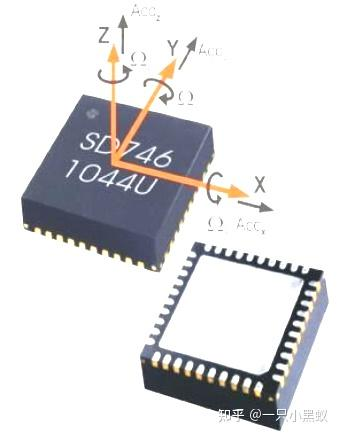
\includegraphics[width=0.3\textwidth]{p1.jpg}
    \caption{IMU示意图}
\end{figure}
\subsection{\heiti\bfseries 机器学习算法}
实验采用TensorFlow高级API Keras构建一个序贯（Sequential）模型。这是一个典型的多层感知机（MLP），其结构如下：

输入层：隐式定义，接收714个归一化后的特征值。

第一个隐藏层：包含50个神经元的全连接层（Dense Layer），使用ReLU（Rectified Linear Unit）作为激活函数。

第二个隐藏层：包含15个神经元的全连接层，同样使用ReLU激活函数。

输出层：包含2个神经元（对应两种手势）的全连接层，使用Softmax作为激活函数。Softmax函数将输出层的原始分数（logits）转换为一个概率分布，每个神经元的输出值表示对应手势的预测置信度。

\section{\heiti\bfseries 实验目的}
利用 Arduino 实现手势识别。

\section{\heiti\bfseries 实验任务}
\begin{enumerate}
    \item 手势训练数据采集
    \item 机器学习模型训练
    \item 模型部署与手势识别验证
\end{enumerate}

\section{\heiti\bfseries 实验步骤}
\subsection{\heiti\bfseries 手势训练数据采集}
\begin{enumerate}
\item 在 Arduino IDE 中，打开IMU\_Capture.ino。
\item 将程序编译并上传至Arduino Nano 33 BLE Sense开发板 。
\item 为熟悉数据特征，可先打开串口绘图仪 (Tools -> Serial Plotter) 。按下按钮并执行手势，观察实时输出的传感器数据波形图 。完成后关闭串口绘图仪 。
\begin{figure}[H]
    \centering
    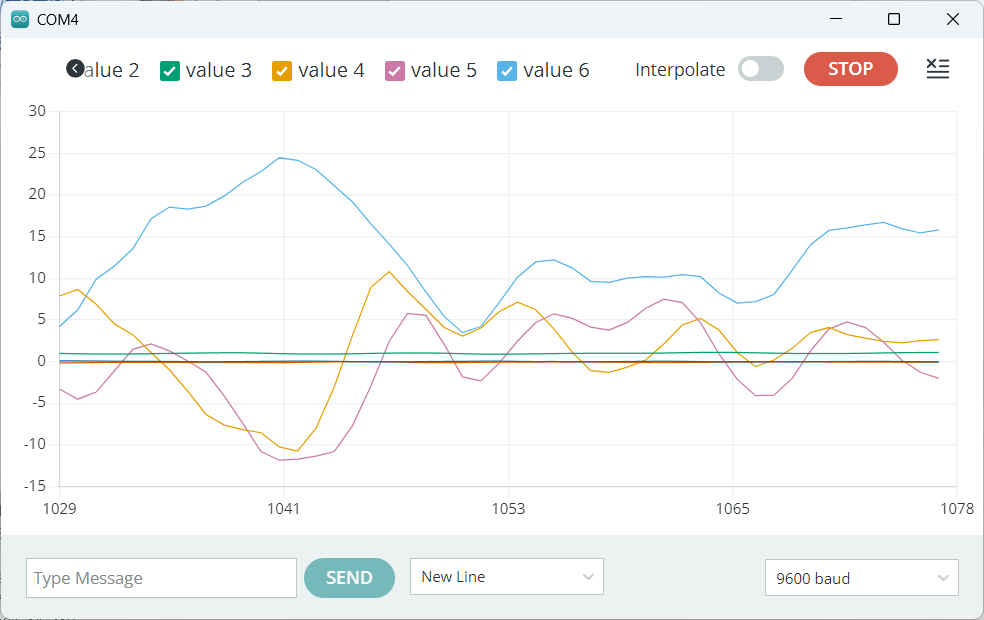
\includegraphics[width=0.8\textwidth]{p3.png}
    \caption{串口绘图仪查看数据示意图}
\end{figure}
\item 打开串口监视器 (Tools -> Serial Monitor) 。
\item {采集“挥拳 (punch)”手势数据}：按下按钮，然后做出挥拳手势 。重复此操作约10次以收集足够的数据 。
\item 将串口监视器中输出的所有数据从头到尾完整地复制,
并粘贴到一个新的文本文件中，命名为 punch\_new.csv。
\item {采集“弯曲 (flex)”手势数据}：再次打开串口监视器，按下按钮，然后做出弯曲手势 。同样重复约10次 。
\item 将串口监视器中输出的所有数据复制并粘贴到一个新的文本文件中，命名为 flex\_new.csv 。
\end{enumerate}
\begin{figure}[H]
    \centering
    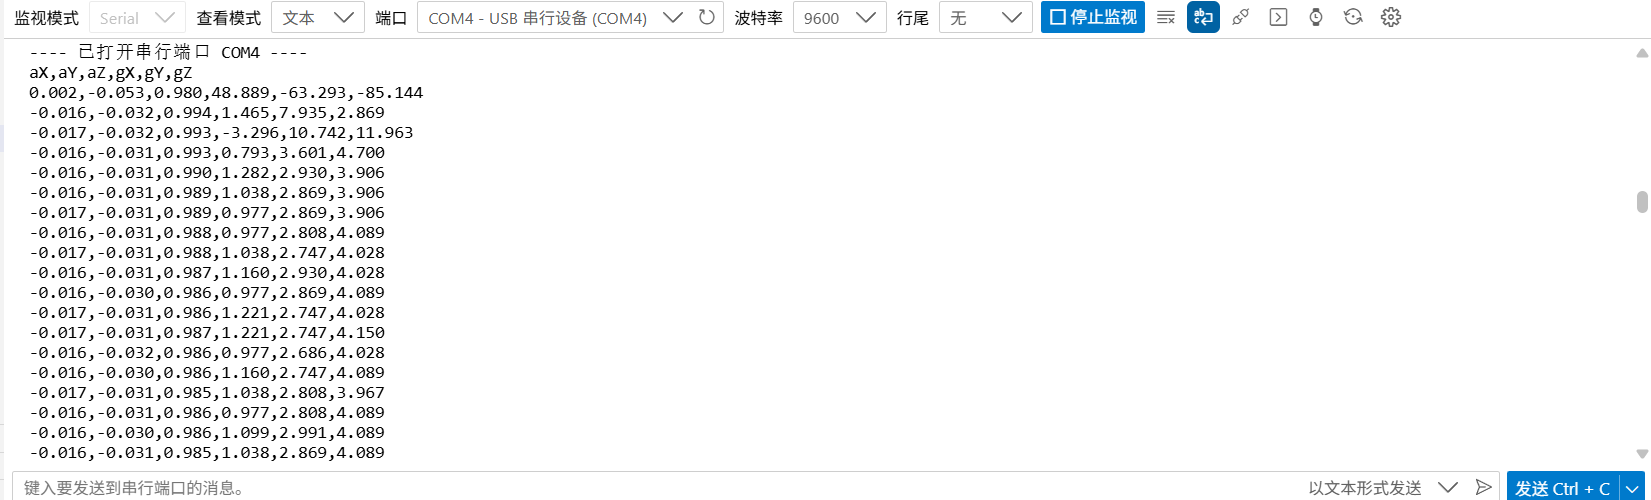
\includegraphics[width=1\textwidth]{p4.png}
    \caption{串口监视器查看数据示意图}
\end{figure}

\subsection{\heiti\bfseries 使用提供的数据集进行机器学习模型训练}

\subsubsection{\heiti\bfseries 训练步骤}

\begin{enumerate}
    \item 打开 arduino\_tinyml\_workshop.ipynb文件
    \item 依次执行笔记本中的代码单元格：
    \begin{itemize}
    \item {Setup Python Environment}：运行此单元以安装 TensorFlow 等必要的 Python 库。
    \item {Parse and prepare the data}：运行此单元以加载、解析、归一化并分割数据集。代码会将数据分为 60\% 的训练集、20\% 的测试集和 20\% 的验证集。
    \item {Build \& Train the Model}：运行此单元以构建神经网络模型并进行600个周期的训练。
    \end{itemize}
    
\end{enumerate}

\subsubsection{\heiti\bfseries 数据可视化}
\begin{figure}[H]
        \centering
        \subcaptionbox{Acceleration (G)}[0.45\textwidth][c]{
            \centering
            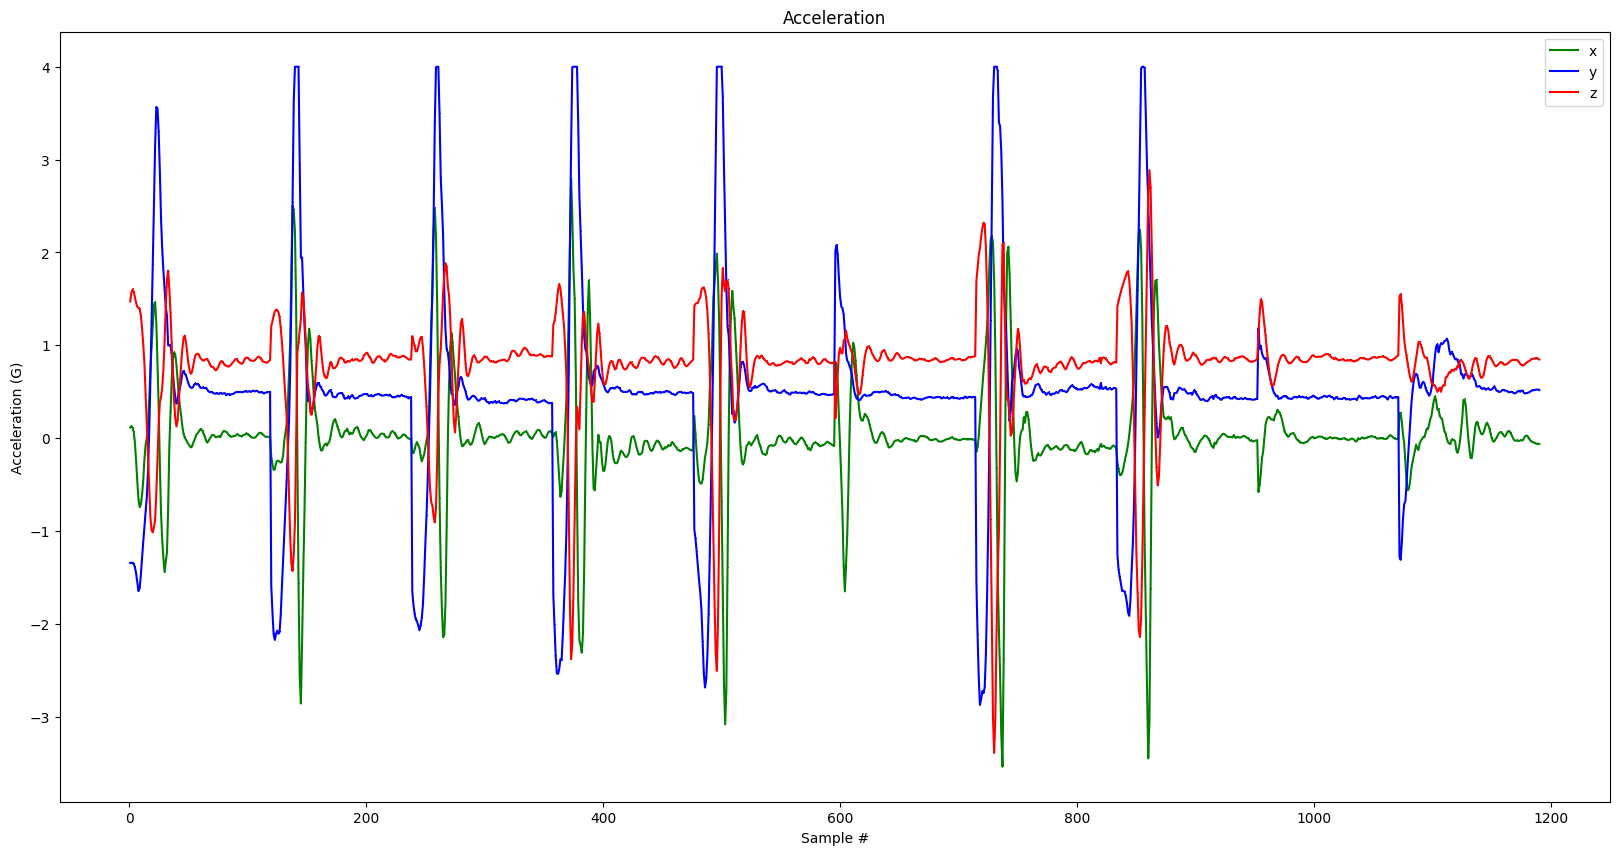
\includegraphics[width=0.4\textwidth]{p16.png}
             
        }%
        \hspace{0.5cm} 
        \subcaptionbox{Gyroscope (deg/sec)}[0.45\textwidth][c]{
            \centering
            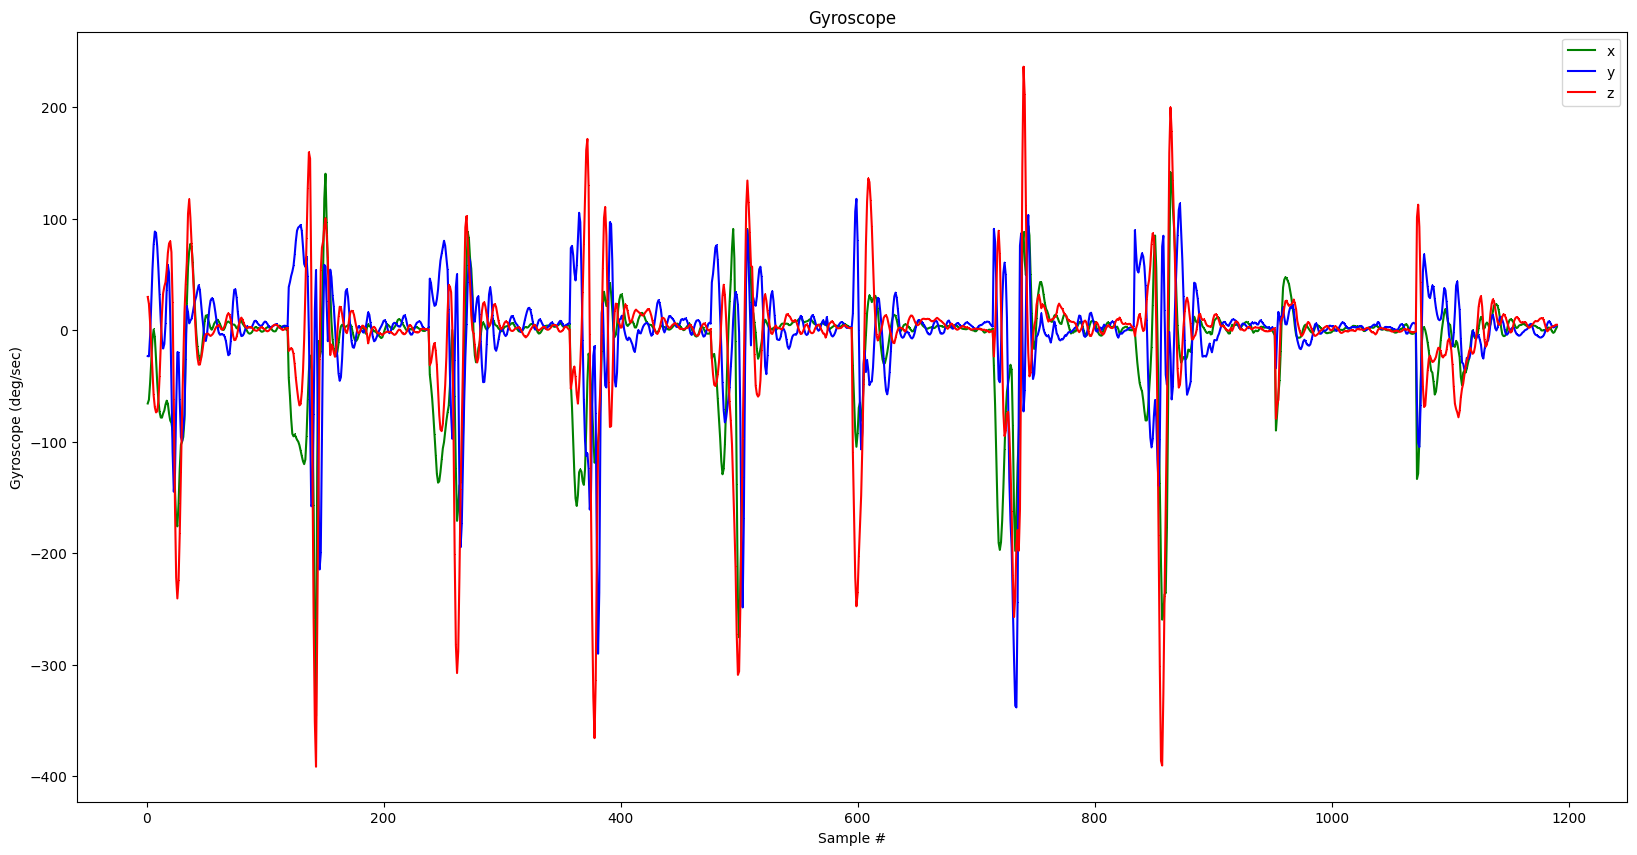
\includegraphics[width=0.4\textwidth]{p17.png}
             
        } 
        \caption{punch数据可视化}
         
    \end{figure}

\subsubsection{\heiti\bfseries 训练结果}

\begin{figure}[H]
        \centering
        \subcaptionbox{Training and validation loss}[0.33\textwidth][c]{
            \centering
            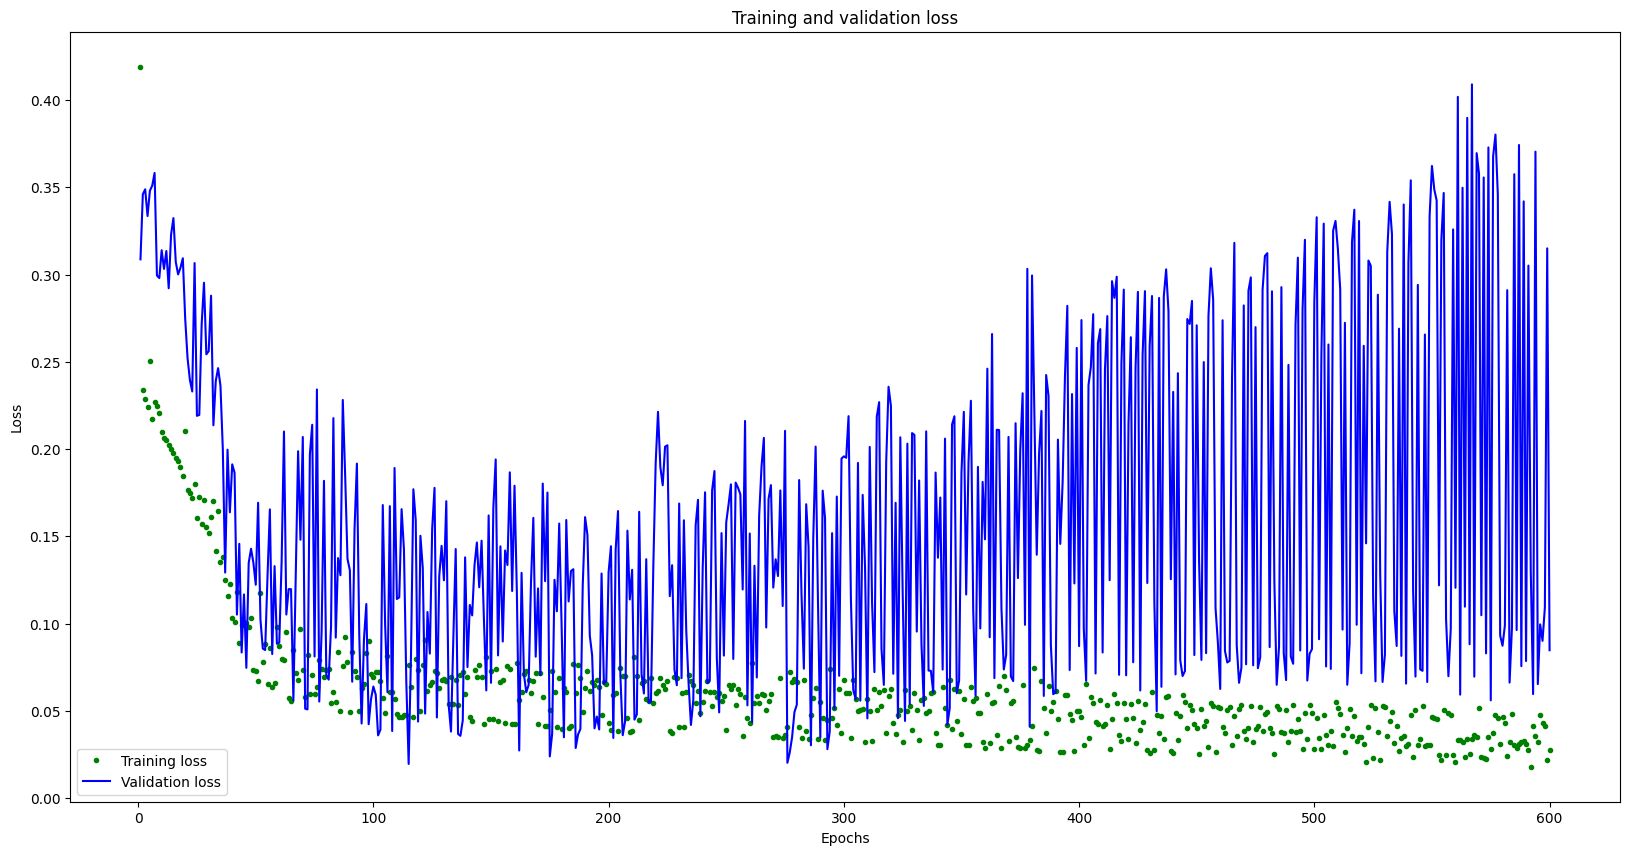
\includegraphics[width=0.32\textwidth]{p7.png}
             
        }%
            \subcaptionbox{Skip start}[0.33\textwidth][c]{
            \centering
            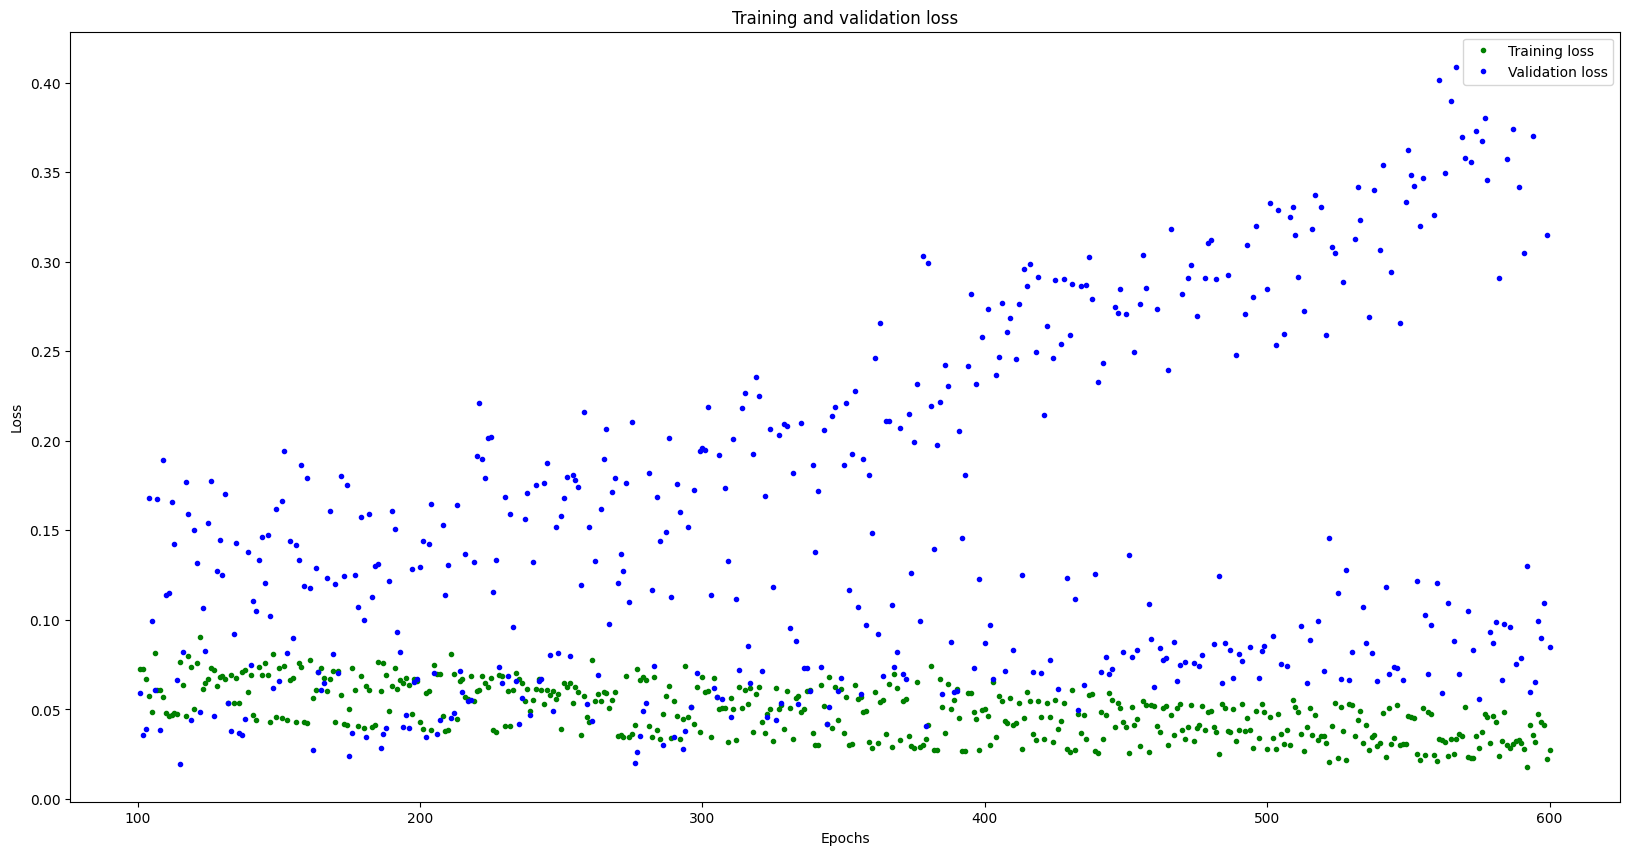
\includegraphics[width=0.32\textwidth]{p9.png}
             
        }%
            \subcaptionbox{Training and validation mae}[0.33\textwidth][c]{
            \centering
            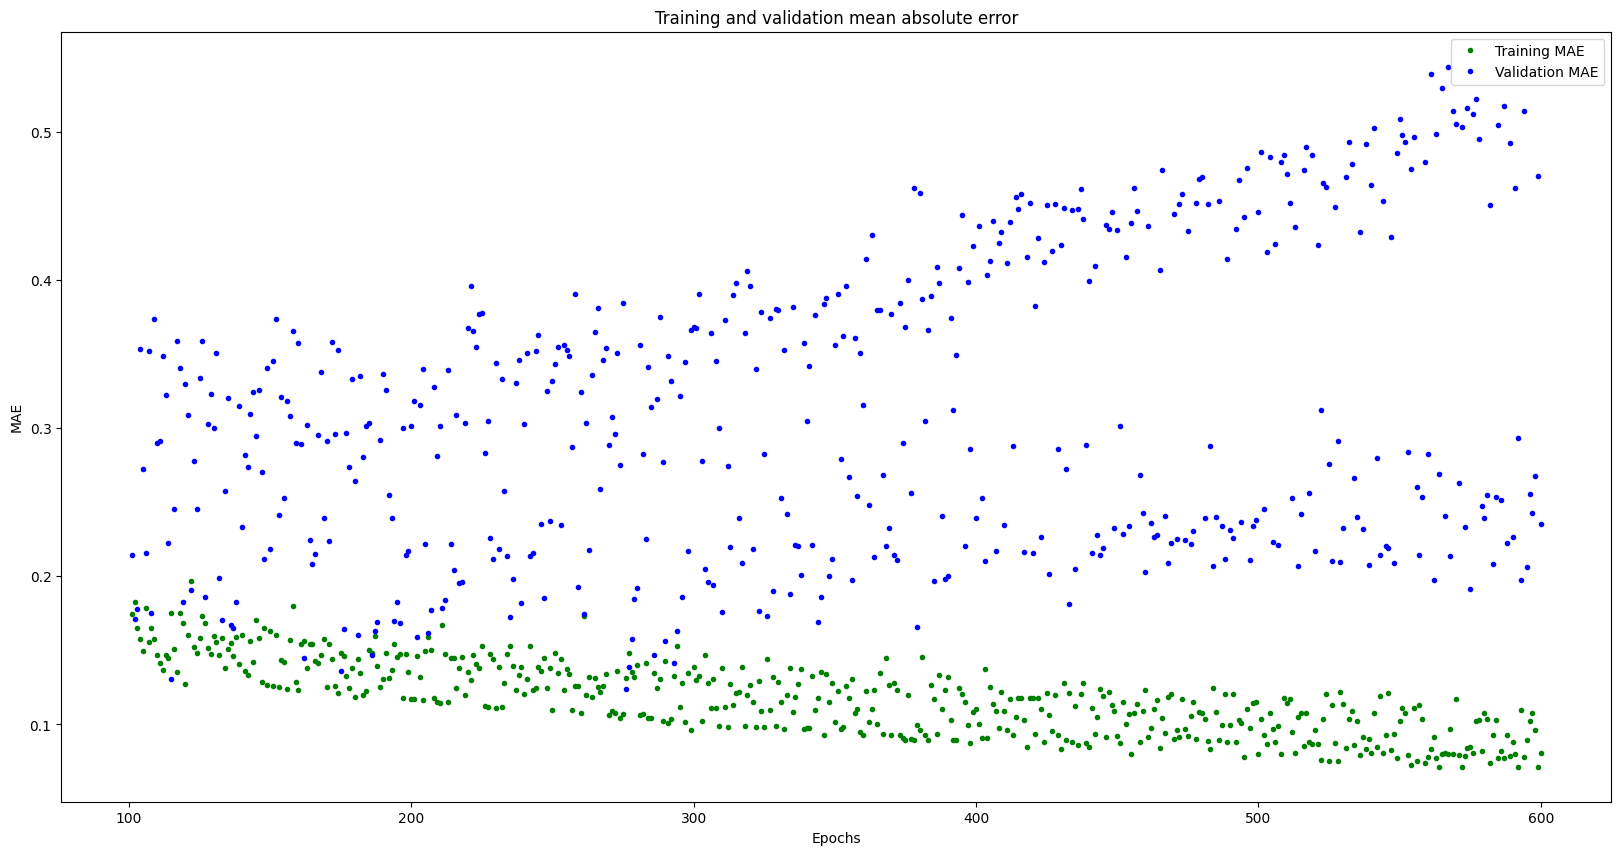
\includegraphics[width=0.32\textwidth]{p11.png}
             
        }%
        \caption{训练结果}
         
\end{figure}

\subsubsection{\heiti\bfseries 实验结论}
\begin{enumerate}
    \item {\heiti\bfseries 模型收敛趋势良好}：从绿色散点（训练损失）可以看出，随着训练周期的增加，损失值从最初的约0.23迅速且持续地下降，最终趋近于0.0。这表明模型很好地学习了训练数据的特征，成功拟合了训练样本。
    \item {\heiti\bfseries 存在明显的过拟合 (Overfitting) 现象}：在训练初期（约前100个周期），验证损失（蓝色线条）随着训练损失一同快速下降，说明模型在开始阶段学习到了普适的规律。
然而，在大约100-150个周期之后，训练损失仍在持续降低，但验证损失不再呈现稳定的下降趋势，反而开始出现剧烈且无规律的震荡，并且其值整体上远高于训练损失。
这种训练损失很低、但验证损失很高且不稳定的现象是典型的过拟合标志。这意味着模型过度学习了训练数据中的细节和噪声，而没有学到足够通用的模式，导致其在新（验证）数据上的表现不佳。
    \item {\heiti\bfseries 验证过程表现出高方差 (High Variance)}：蓝色线条（验证损失）的剧烈波动表明模型在不同批次的验证数据上表现非常不稳定

\end{enumerate}

\subsubsection{\heiti\bfseries 模型优化}
为了改善过拟合问题，选择如下代码简化模型结构，减少隐藏层神经元数量，通过对比可以发现，简化后的模型在训练和验证集上的表现更加接近，验证损失曲线更加平滑，说明模型的泛化能力有所提升，过拟合现象得到缓解。

\begin{lstlisting}[language=python, caption=原先的build代码]
    # build the model and train it
    model = tf.keras.Sequential()
    model.add(tf.keras.layers.Dense(50, activation='relu'))
    model.add(tf.keras.layers.Dense(15, activation='relu'))
    model.add(tf.keras.layers.Dense(NUM_GESTURES, activation='softmax'))
    model.compile(optimizer='rmsprop', loss='mse', metrics=['mae'])
    history = model.fit(inputs_train, outputs_train, epochs=600, batch_size=4, validation_data=(inputs_validate, outputs_validate))
\end{lstlisting}

\begin{lstlisting}[language=python, caption=简化后的build代码]
    # build the model and train it
    model = tf.keras.Sequential()
    model.add(tf.keras.layers.Dense(10, activation='relu'))
    model.add(tf.keras.layers.Dense(5, activation='relu'))
    model.add(tf.keras.layers.Dense(NUM_GESTURES, activation='softmax'))
    model.compile(optimizer='rmsprop', loss='mse', metrics=['mae'])
    history = model.fit(inputs_train, outputs_train, epochs=600, batch_size=4, validation_data=(inputs_validate, outputs_validate))
\end{lstlisting}


\begin{figure}[H]
        \centering
        \subcaptionbox{Training and validation loss}[0.33\textwidth][c]{
            \centering
            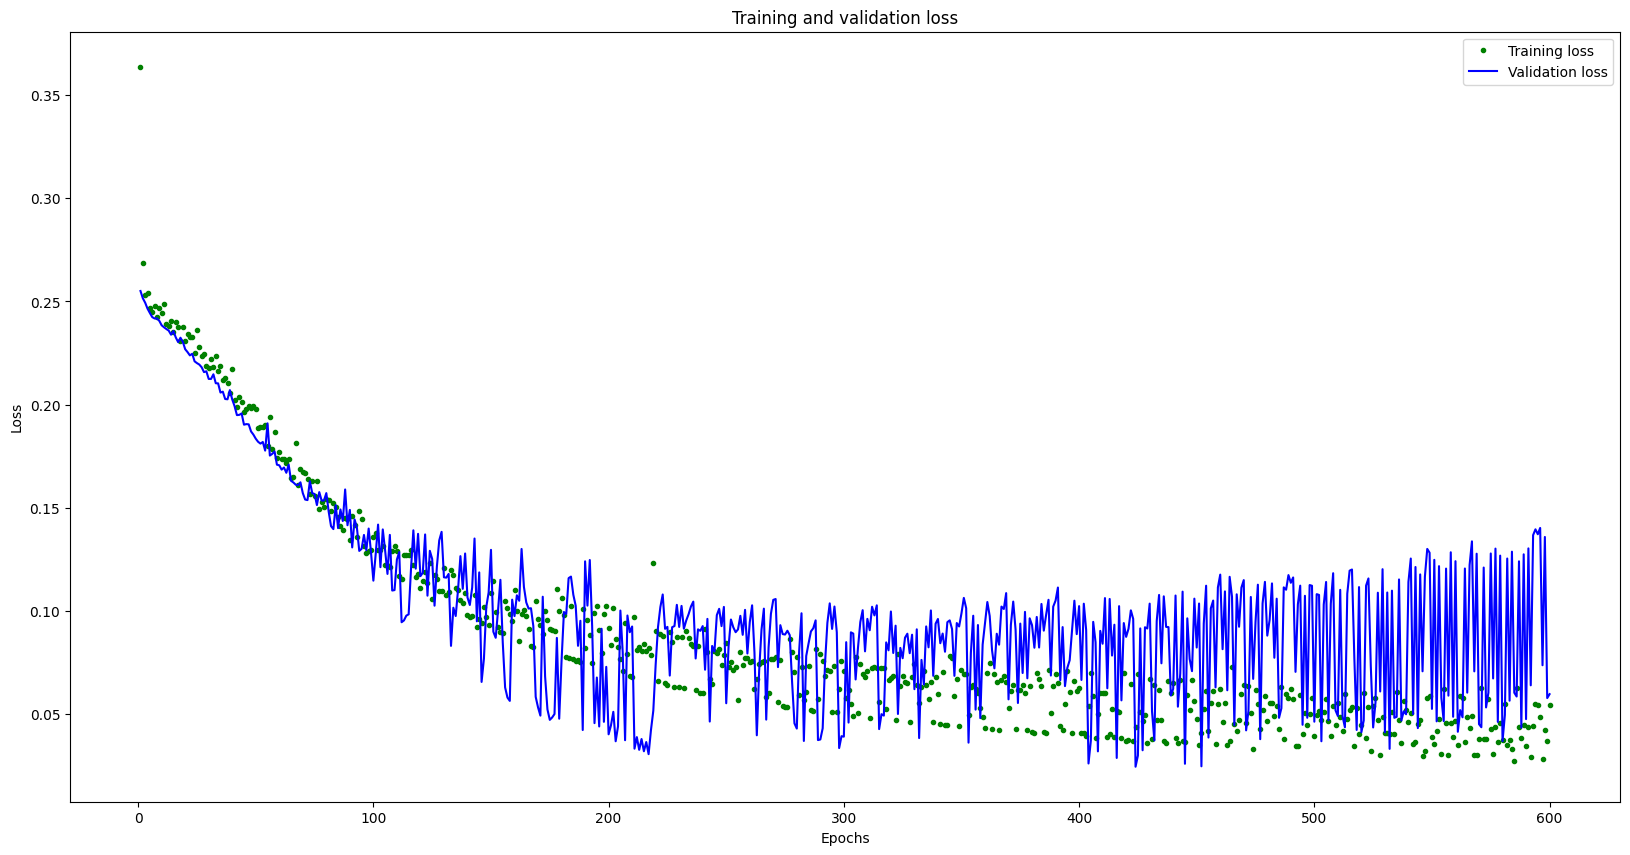
\includegraphics[width=0.32\textwidth]{p8.png}
             
        }%
            \subcaptionbox{Skip start}[0.33\textwidth][c]{
            \centering
            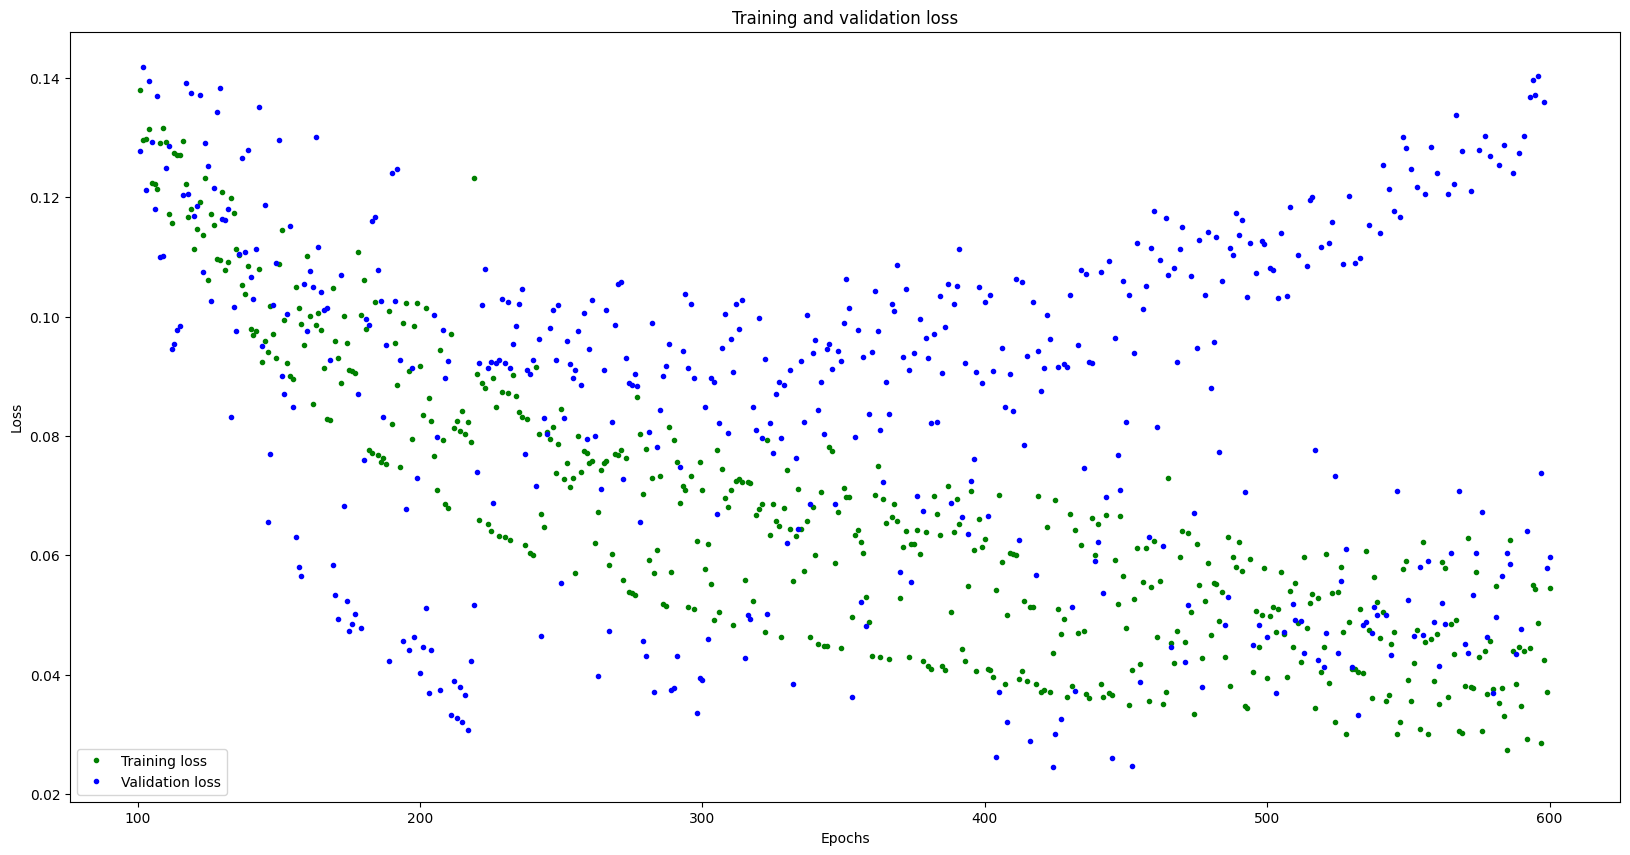
\includegraphics[width=0.32\textwidth]{p10.png}
             
        }%
            \subcaptionbox{Training and validation mae}[0.33\textwidth][c]{
            \centering
            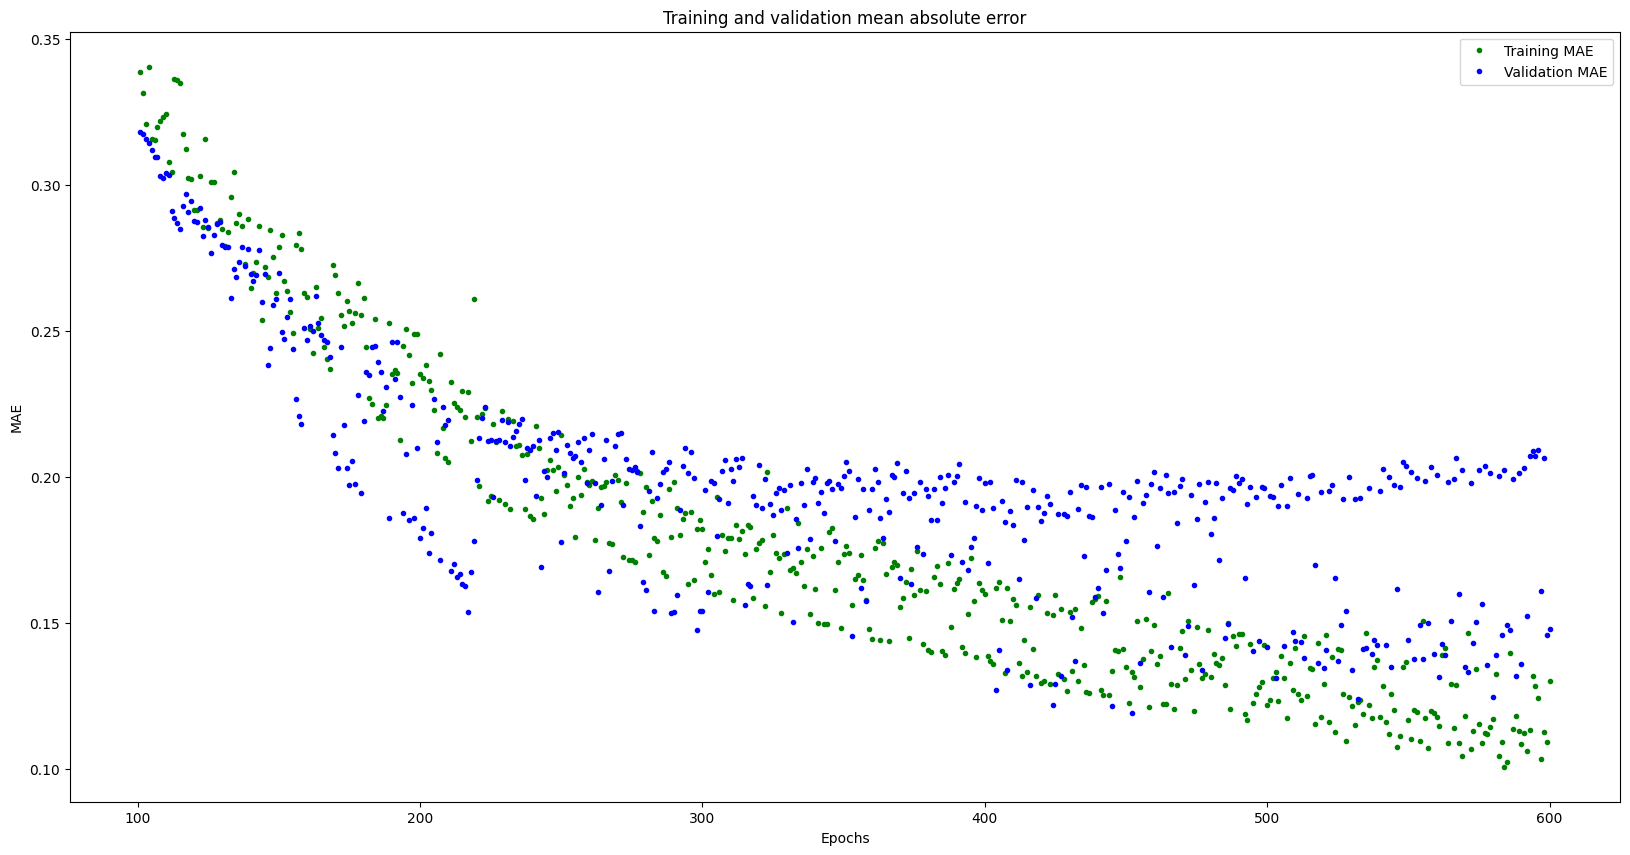
\includegraphics[width=0.32\textwidth]{p12.png}
             
        }%
        \caption{优化后结果}
         
\end{figure}

\begin{figure}[H]
    \centering
    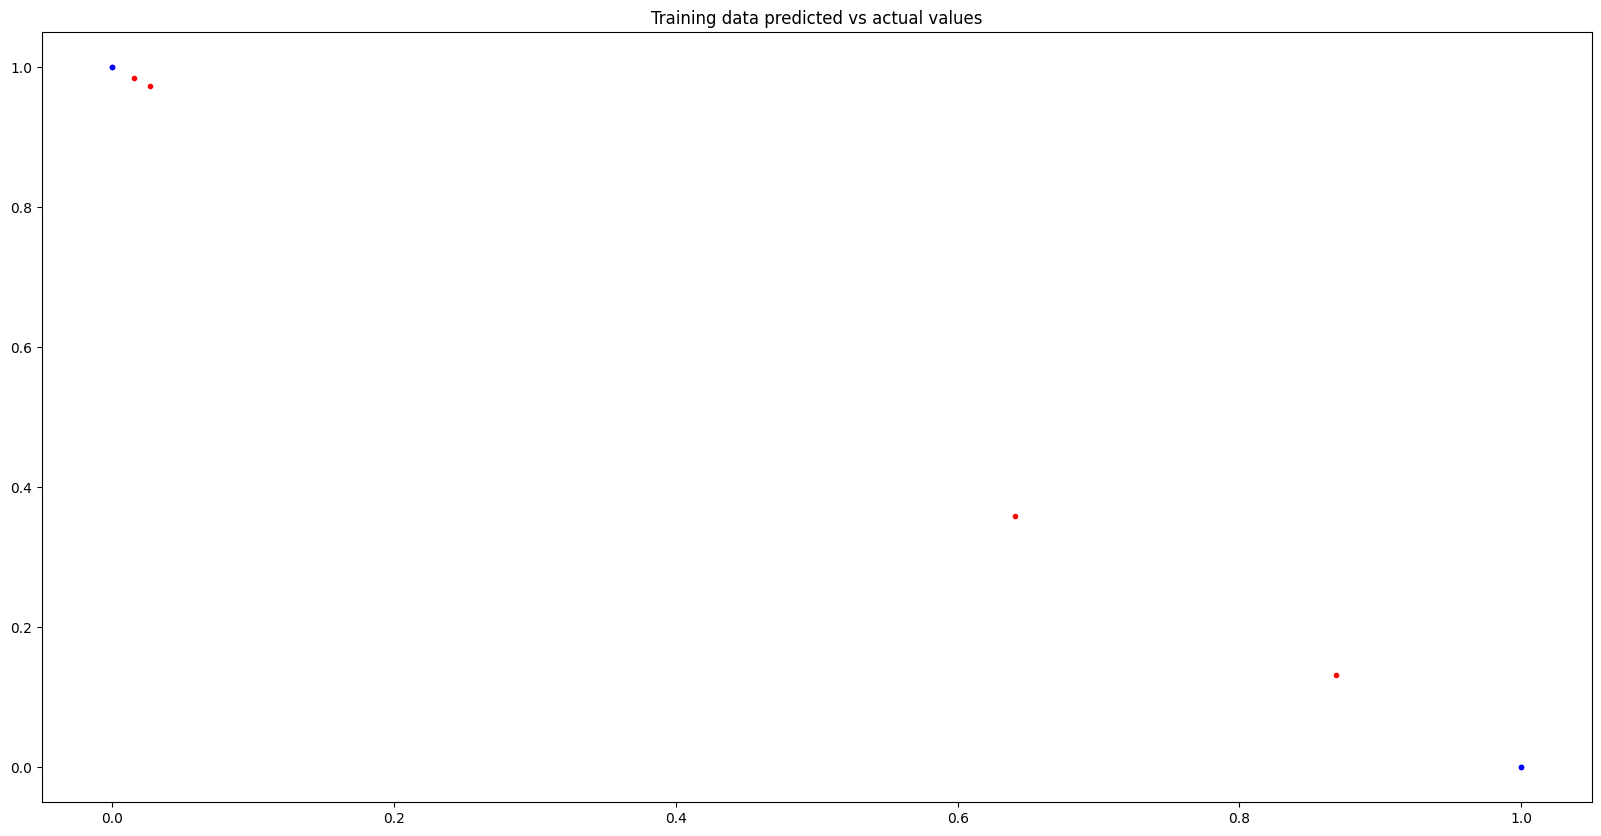
\includegraphics[width=0.6\textwidth]{p13.png}
    \caption{优化后Training data predicted vs actual values}
\end{figure}

\subsection{\heiti\bfseries 使用自己采集的数据集进行训练}

将Build \& Train the Model处代码更改回原先的代码

更改Graph Data (optional)中代码如下
\begin{lstlisting}[language=python, caption=原先的build代码]
    filename = "punch_new.csv"
\end{lstlisting}

更改Parse and prepare the data处代码如下
\begin{lstlisting}[language=python, caption=原先的build代码]
GESTURES = [
    "punch_new",
    "flex_new",
]
\end{lstlisting}

以采用自己采集的数据集进行测试
\subsubsection{\heiti\bfseries 数据可视化}
\begin{figure}[H]
        \centering
        \subcaptionbox{Acceleration (G)}[0.45\textwidth][c]{
            \centering
            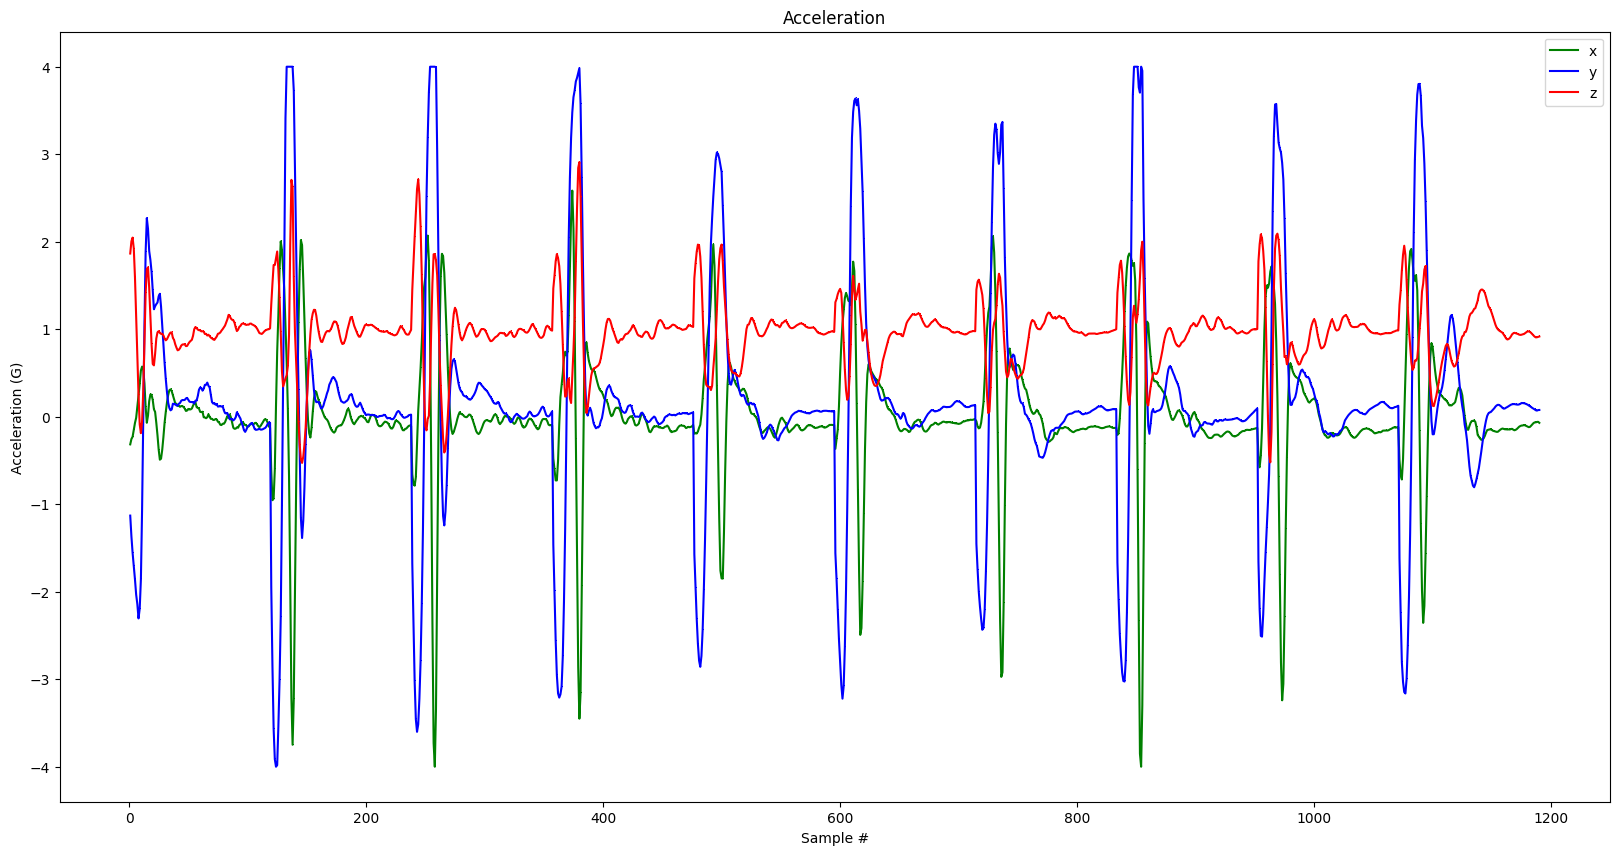
\includegraphics[width=0.4\textwidth]{p5.png}
             
        }%
        \hspace{0.5cm} 
        \subcaptionbox{Gyroscope (deg/sec)}[0.45\textwidth][c]{
            \centering
            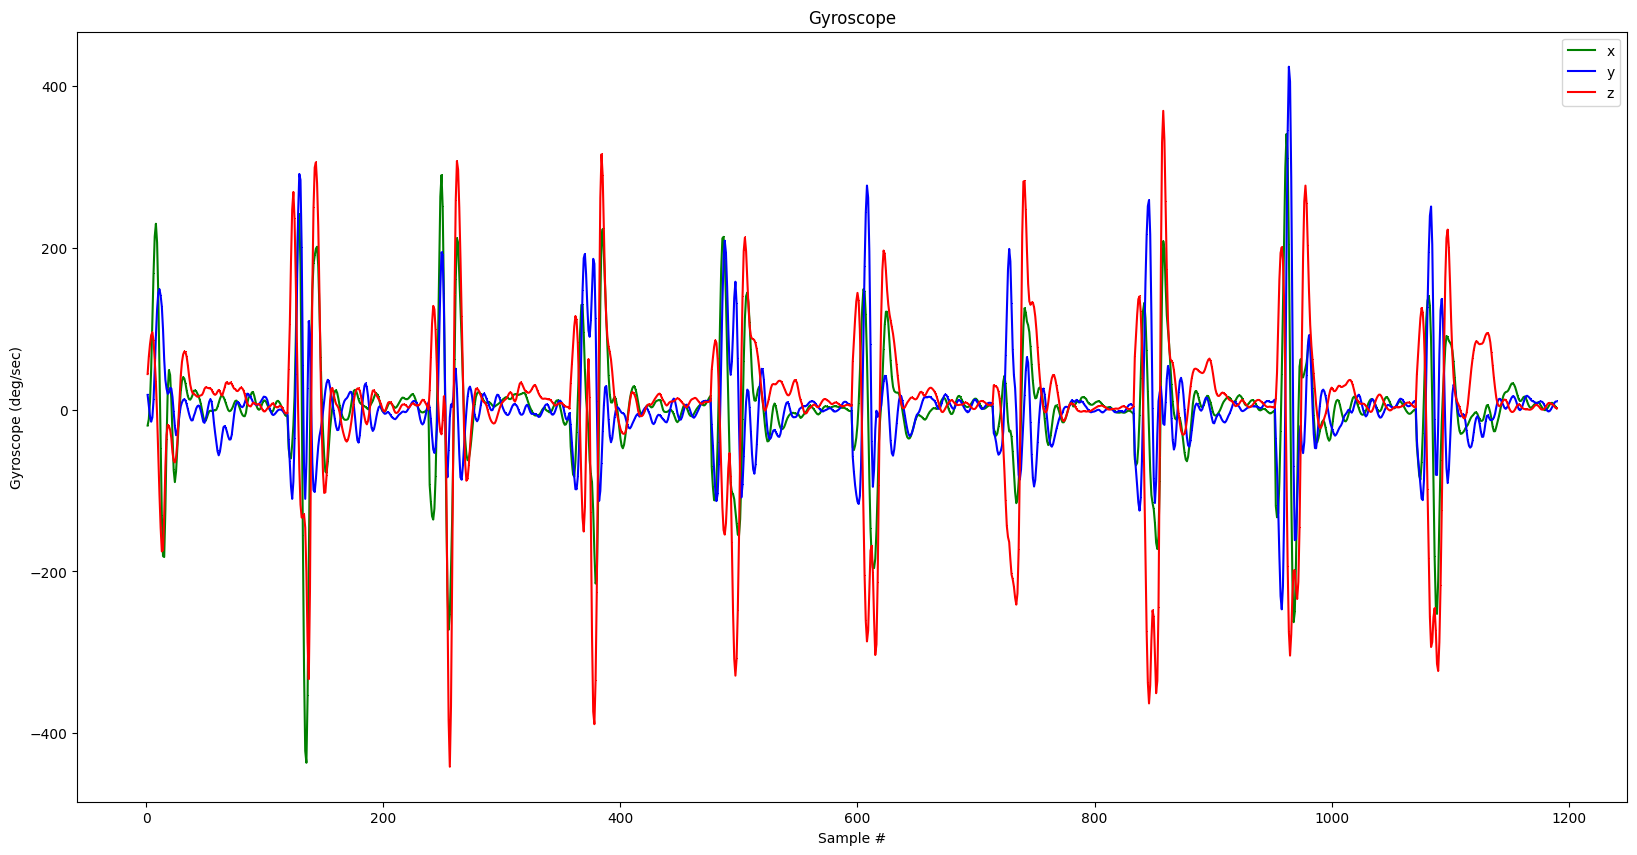
\includegraphics[width=0.4\textwidth]{p6.png}
             
        } 
        \caption{punch数据可视化}
         
    \end{figure}

\subsubsection{\heiti\bfseries 训练结果}
\begin{figure}[H]
    \centering
    \subcaptionbox{Training and validation loss}[0.33\textwidth][c]{
        \centering
        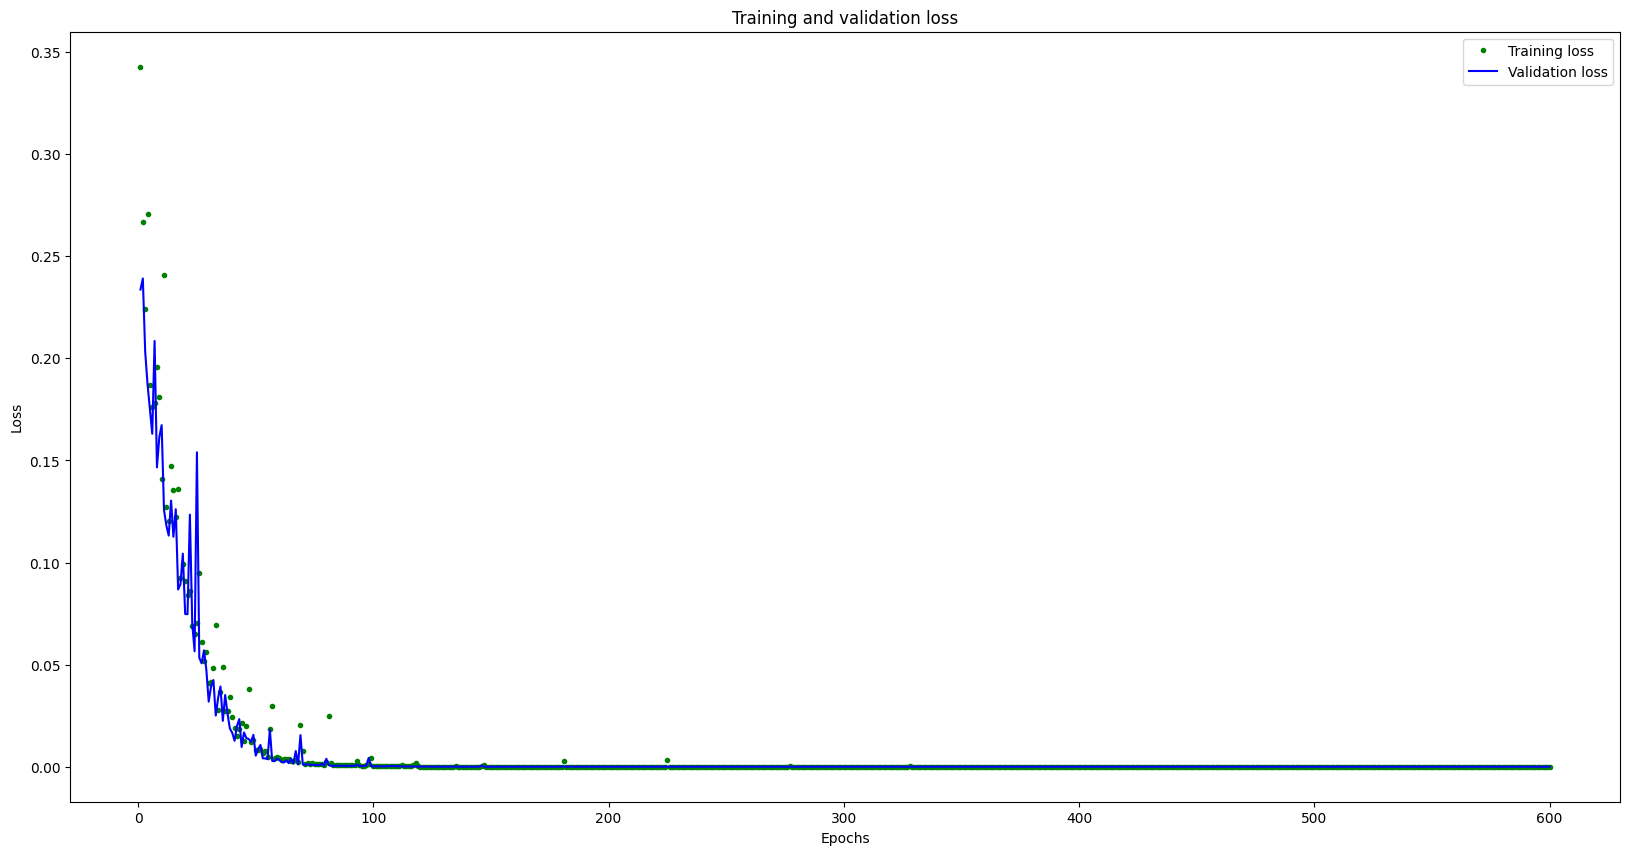
\includegraphics[width=0.32\textwidth]{p18.png}
            
    }%
        \subcaptionbox{Skip start}[0.33\textwidth][c]{
        \centering
        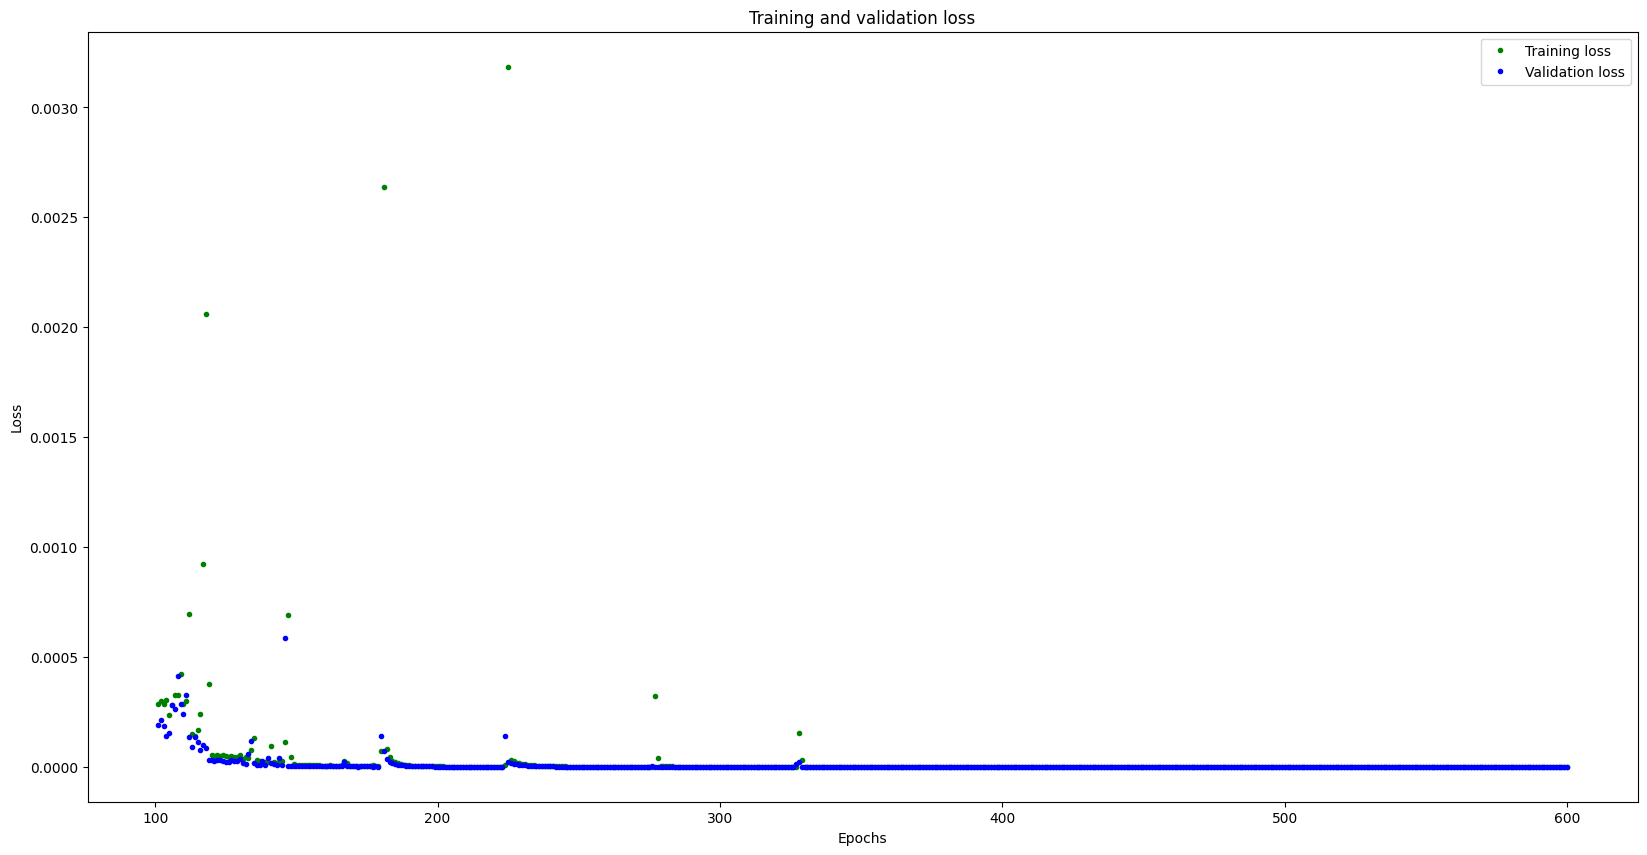
\includegraphics[width=0.32\textwidth]{p19.png}
            
    }%
        \subcaptionbox{Training and validation mae}[0.33\textwidth][c]{
        \centering
        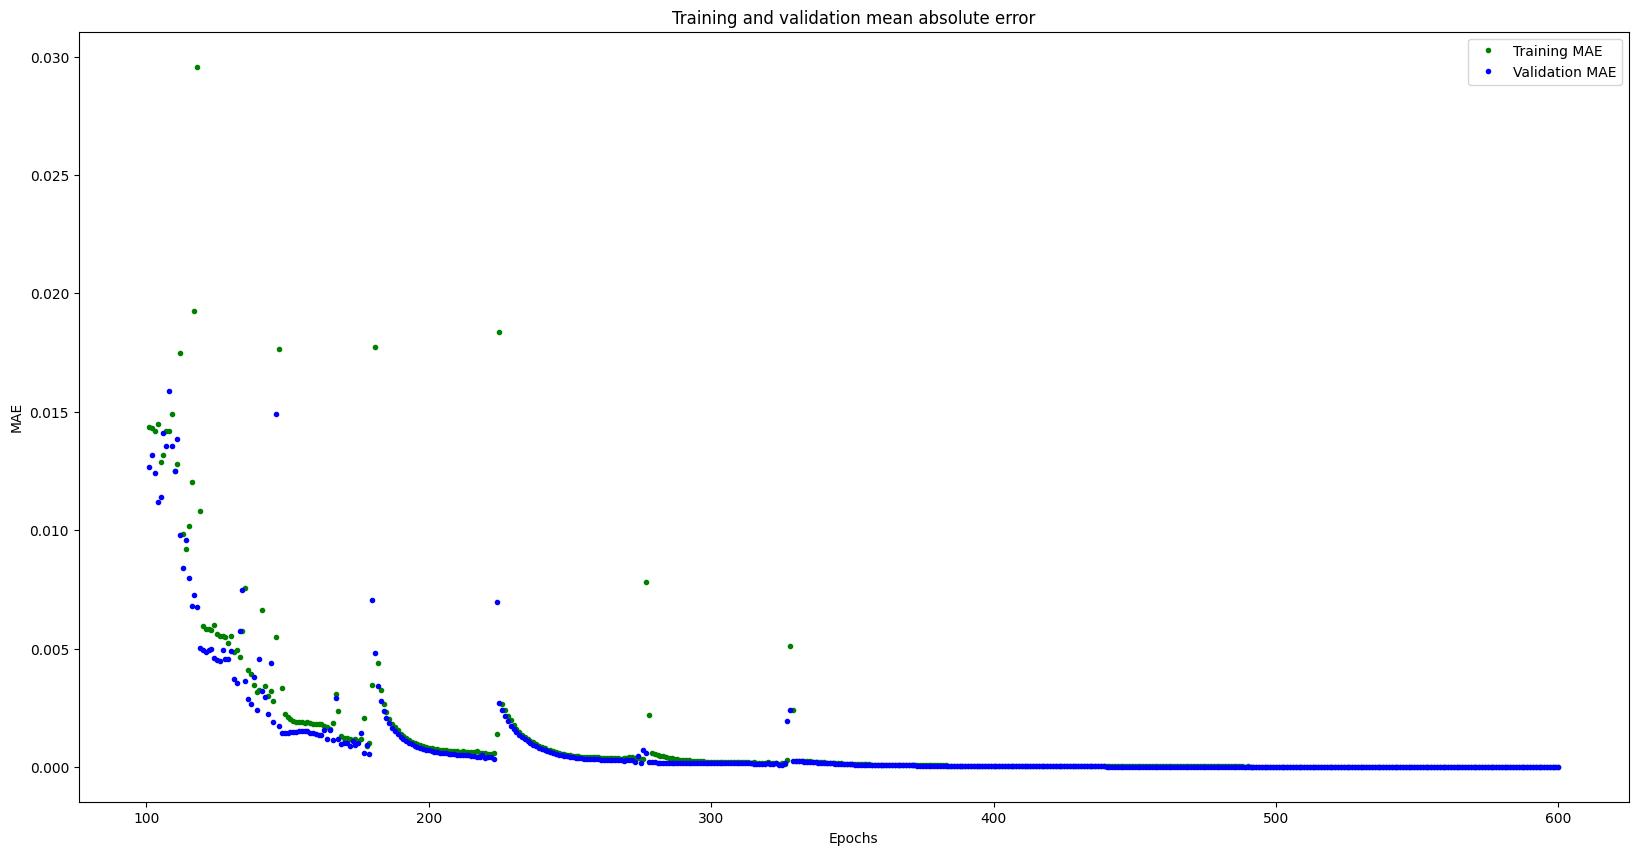
\includegraphics[width=0.32\textwidth]{p20.png}
            
    }%
    \caption{训练结果}
    
\end{figure}
  \begin{figure}[H]
        \centering
        \begin{minipage}[b]{0.6\linewidth}
            \centering
            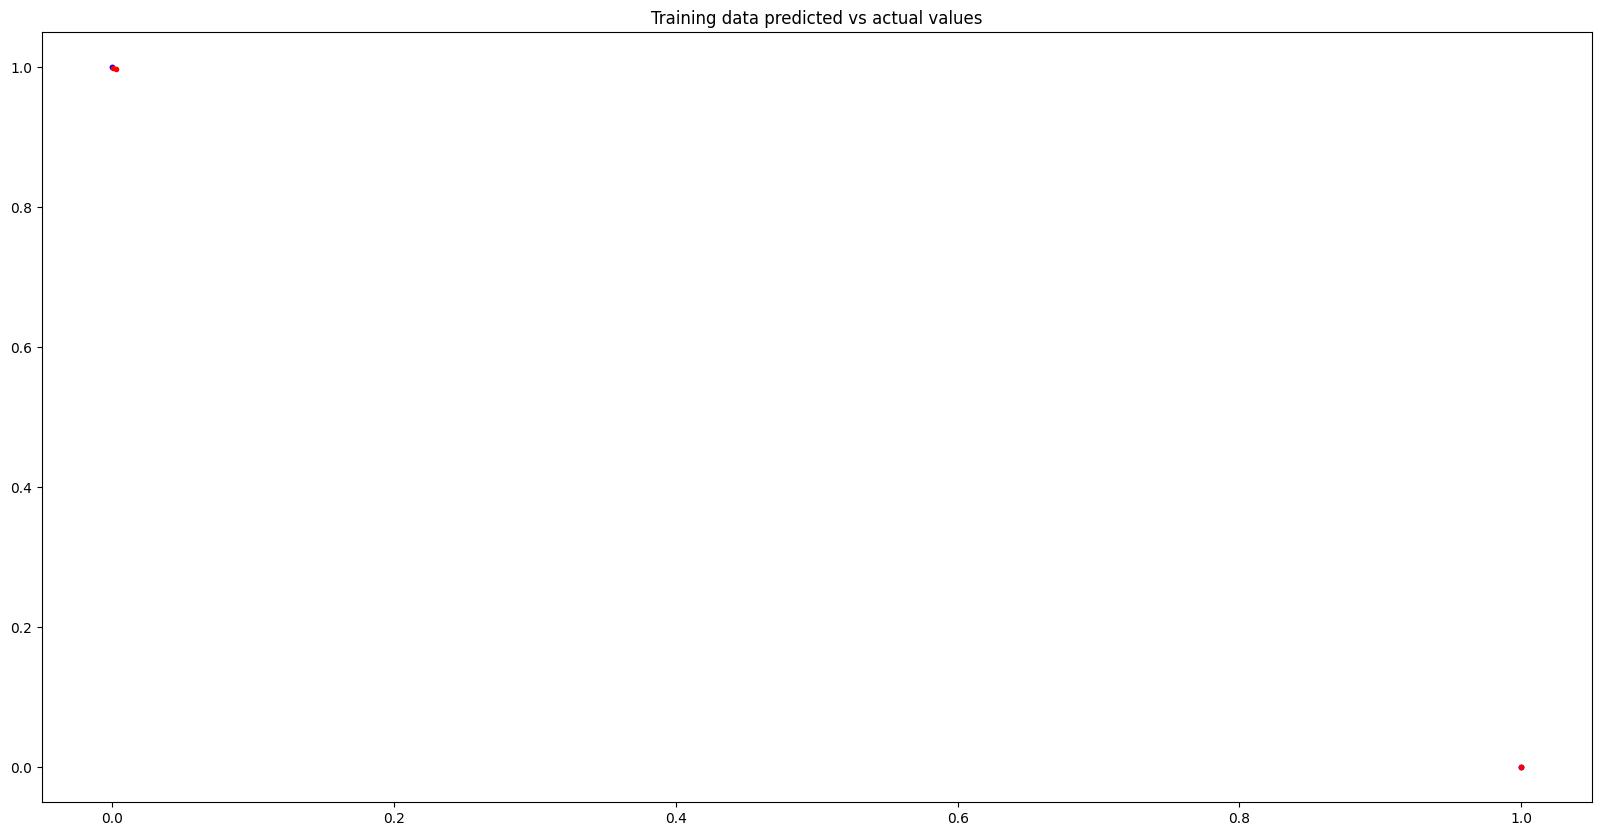
\includegraphics[width=0.9\textwidth]{p21.png}
      
        \end{minipage}%
        \begin{minipage}[b]{0.2\linewidth}
            \centering
            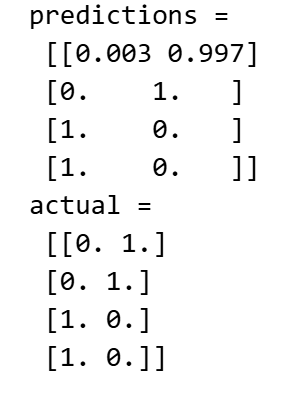
\includegraphics[width=0.9\textwidth]{p22.png}

        \end{minipage}
        \caption{Training data predicted vs actual values}
    \end{figure}

\subsubsection{\heiti\bfseries 实验结论}
    从Figure 9中可以看出，训练损失（Training loss）与验证损失（Validation loss）曲线在整个训练过程中高度重合，且均能快速、稳定地收敛至一个非常低的值。这表明模型成功学习到了自采集数据的特征。

    从Figure 10中可以看出，红点与两端蓝点非常接近，说明在测试集中，预测值与实际值高度一致，模型训练良好。

    {\heiti\bfseries 实验表明，优化训练数据质量有时候远比优化模型结构实用，合适的数据可以让一个简单的模型达到很好的效果。}
\subsection{\heiti\bfseries 模型部署与手势识别验证}
\subsubsection{\heiti\bfseries 实验步骤}
\begin{enumerate}
    \item 将上一步生成的 C 头文件内容替换项目中的模型文件
    \item 将最终的识别程序 `demo3\_2\_IMU\_Classifier` 上传到 Arduino 开发板。
    \item 打开串口监视器，执行相应手势，观察模型输出的每个手势的置信度分数（0到1之间），验证手势识别的准确性。
\end{enumerate}
\subsubsection{\heiti\bfseries 实验结果}
    如下，分别进行三次punch动作与flex动作，发现置信度分数非常高，说明均能被正确识别
  \begin{figure}[H]
        \centering
        \begin{minipage}[b]{0.5\linewidth}
            \centering
            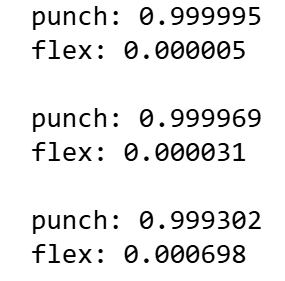
\includegraphics[width=0.9\textwidth]{p14.png}
              \caption{Punch动作识别结果}
        \end{minipage}%
        \begin{minipage}[b]{0.5\linewidth}
            \centering
            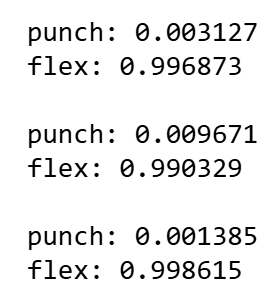
\includegraphics[width=0.9\textwidth]{p15.png}
              \caption{Flex动作识别结果}
        \end{minipage}
                \caption{动作识别结果}
    \end{figure}

\section{\heiti\bfseries 实验总结}
    该实验成功地在边缘计算设备（Arduino Nano 33 BLE Sense）上，通过IMU（惯性测量单元）实现了手势的实时识别。

    实验表明了训练数据质量和代表性的重要性。一份准确、能够真实反映实际应用场景的数据集，可以让一个相对简单的模型达到优异的性能，
\end{document}
